\documentclass{article}
\usepackage{graphicx}
\usepackage{hyperref}
\usepackage{url}

\setlength{\parskip}{1em}

\begin{document}


\section{Visualizing Output}

Currently, ICE features two plugins for visualizing and plotting simulation
output data:

\textbf{VisIt Tools} - An interactive 3D visualization tool for rendering
meshes, scalar plots, contour plots, and more. 

\textbf{CSV Plotting Tools} - A customizable, 2D data plotting utility for data 
from .csv files.

\subsection{Installation and Configuration}

The CSV Plotting Tools require no additional software or preparation before use.
The VisIt Tools need both an instance of VisIt and a connection between ICE and
the VisIt session.

\subsubsection{VisIt Installation} 

Before preparing ICE,
\href{https://wci.llnl.gov/simulation/computer-codes/visit/}{VisIt}, developed
by Lawrence Livermore National Laboratory, must be downloaded. This must be
version 2.8.2, and does not need to be on the same machine that ICE is installed
on, as ICE is capable of launching a VisIt session on a remote machine. Make
note of the folder where you installed VisIt for use in the next step.

\subsubsection{Configuring the VisIt Connection}

Once VisIt is installed, ICE must connect to a VisIt session in order to provide
data visualization. There are two different parts of ICE which connect with
VisIt, both providing slightly different functionalities. These are the Plot
Editor, which is slightly more user friendly, and the Visualization Perspective,
which allows for arbtrary Python commands to be sent to the VisIt client. 

\paragraph{Connecting for the Plot Editor}

This process will set up a default connection to VisIt in the ICE Preferences
page, and so only needs to be performed once. After creating the connection, ICE
will launch and connect with VisIt each time it is started.

To set the connection, select Window $\rightarrow$ Preferences in ICE's toolbar. Then
select Visualization $\rightarrow$ VisIt in the tree of the Preferences page. 

\begin{center}
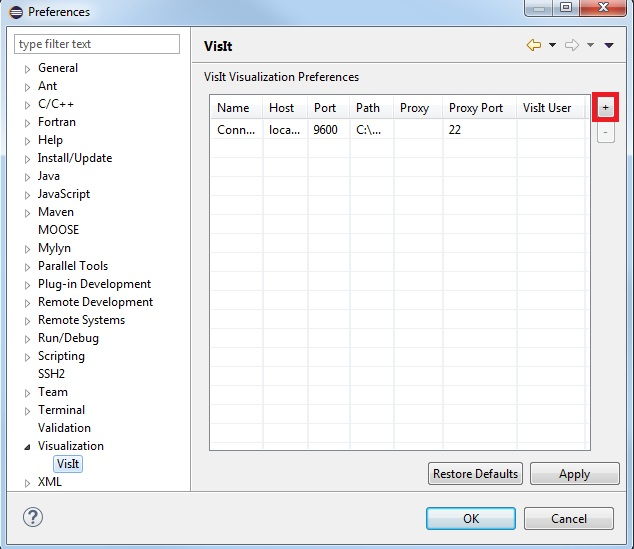
\includegraphics[width=12cm]{images/VisItPreferencePage_ICE}
\end{center}

Press the new row button, the button with a "+" symbol in the upper right,
highlighted in the image above. You can then click on each of the cells of the
new row to edit them. The default values automatically supplied by ICE should
be fine for most users. However, two fields may need to be changed:

\textbf{Host:} The default value of "localhost" is for connections to local
installations of VisIt on your computer. If you want to launch a remote VisIt
connection, you must change this to the hostname of the machine to connect to.

\textbf{Path:} You need to put the full path to the VisIt folder here. The path
should end with the folder containing the VisIt executable. For example, if
VisIt.exe is in a folder called VisIt 2.9.1, the the path should end in
\textbackslash{}VisIt 2.9.1\textbackslash , not \textbackslash{}VisIt
2.9.1\textbackslash VisIt.exe.

Once finished, press Apply, then OK. ICE will then open VisIt and connect to it.

\paragraph{Connecting for the Visualization Perspective} 

First, open the Visualization perspective. On the main menu bar at the top of
the window, click Window $\rightarrow$ Open Perspective $\rightarrow$
Other\ldots, select Visualization in the fialog that pops up and click OK. Alternatively, you can
also access the same pop-up dialog by clicking the Open Perspective button in
the main toolbar in the upper right-hand corver of the ICE workbench. 

\begin{center}
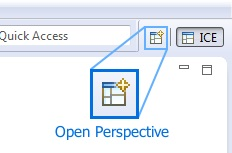
\includegraphics{images/ICE_OpenPerspective}
\end{center}

Now click the Launch VisIt button in the menu bar.

\begin{center}
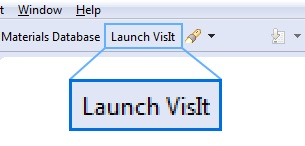
\includegraphics{images/ICE_VisItLaunchButton}
\end{center}

This will open a dialog offering you three options for connecting to VisIt.

\begin{center}
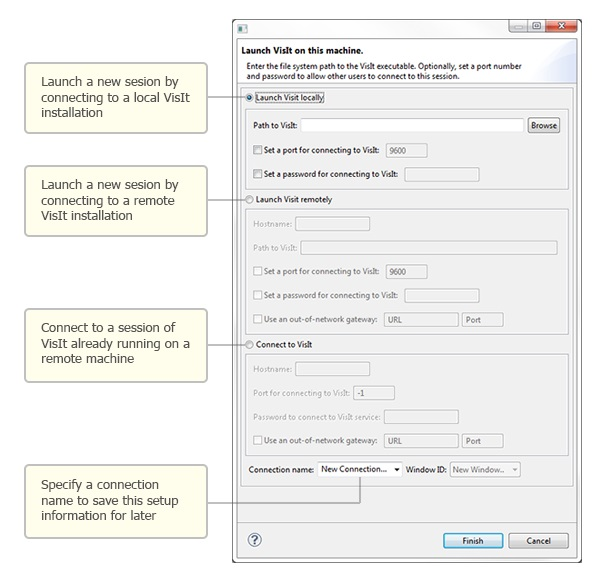
\includegraphics[width=12cm]{images/ICE_VisItLaunchOptions}
\end{center}

1) Launch VisIt locally - If you installed VisIt on your local machine, use the
Browse button to direct ICE to your local installation directory. Using this
method of connecting will launch a new VisIt session. Optionally, you can also
set a port number (default 9600) and--if you want to share your VisIt session
with another user--a password.

2) Launch VisIt remotely - If you installed VisIt on a remote machine, specify
the hostname and full path to the VisIt installation directory. Using this
method of connecting will launch a new VisIt session. Optionally, you can
specify a port number (default 9600) and--if you want to share your VisIt
session with another user--a password. If you need or want to use an external
gateway or proxy to access the remote VisIt installation, you may specify its
URL and port number as well.

3) Connect to VisIt - If you would like to connect to session of VisIt already
running somewhere else, specify the hostname, port number, and password set on
the VisIt session; you will need to obtain this information from the person who
initially launched the VisIt session. If you need or want to use an external
gateway or proxy to access the remote VisIt installation, you may specify its
URL and port number as well.

If you've forgotton where VisIt is installed on Windows, find a shortcut to
VisIt eithero n your desktop or in the start menu. Right-click the shortcut and
open its Properties. The path to the VisIt executable's directoy will be shown
next to Target.

Regardless of which method you choose to connect to VisIt, enter a Connection
name at the bottom of the pop-up dialog. 

If you are connecting to an existing session, specify a Window ID between 1 and
16. Which Window ID you use depends on how you would like to connect to VisIt.
If multiple users connect using the same Window ID, they will all see and be
able to interact with the same VisIt view. However, if you would like multiple
users to each have their own unique session each with its own controls, assign a
unique Window ID to each user. The VisIt installation can support up to 16
unique window IDs at a time.

Once you are done, click the Finish button at the bottom, and ICE should begin
connecting to VisIt.

\subsubsection{Using VisIt}

\paragraph{Plot Editor}

To open a plot editor, first the file must be placed in the Project Explorer.
This view lists files imported into ICE. To access the Project Explorer, use the
the main menu bar at the top of the window and navigate to Window $/rightarrow$
Show View $/rightarrow$ Project Explorer. 

By default, the Project Explorer should automatically import the
ICEFiles/default and ICEFiles/itemDB folders. If it does not, or it you want to
import a different folder into ICE, right click in the Project Explorer and
select Import... from the context menu. Then select General -> File System from
the tree and press the Next button. You can then select directories and/or files
to import into the Project Explorer.

\end{document}
